\genHeader
\label{chap:Learning-Box-to-Dictionary-and-Back-Again}

\requiredTime{1h 30min}

If you're just joining us in this part and are only interested in bidirectional model transformations with \emph{Triple Graph Grammars}, then welcome!
To ensure eMoflon is running correctly however, you should at least work through Part I for the required installation and set-up instructions. We try to assume
as little as possible from the previous parts in the handbook series here, and give appropriate references where necessary.

To briefly review what we have done so far, we have developed Leitner's learning box by specifying its \emph{abstract syntax} and \emph{static
semantics} as a \emph{metamodel}, and finally its \emph{dynamic semantics} via Story Driven Modeling (SDM graph transformations). If the previous sentence could
just as well have been in Chinese\footnote{Replace with Greek if you are chinese.  If you are chinese but speak fluent Greek, then we give up. You get the point
anyway, right?} for you, then please work through Parts II and III.

We realize now however that even though SDMs are crazily cool (don't you forget that!), it is rather unsatisfactory implementing a \emph{bidirectional}
transformation as two unidirectional transformations. If you take a careful and critical look at the concept of forward and the backward transformations, you
should be able to realise the following problems.

\begin{description}
\item[Productivity:] We have to implement two transformations that are really quite similar, \emph{separately}. This doesn't really feel productive.
Wouldn't it be nice to implement one direction such as the forward transformation, then get the backward transformation for free? How about deriving
forward \emph{and} backward transformations from a common joint specification?

\item[Maintainability:] Another, maybe even more important point is that two separate transformations often become a pain to maintain and keep
\emph{consistent}. If the forward transformation is ever adjusted to produce a different target structure, the backward transformation must be updated
appropriately to accommodate the change, and vice-versa.  Again, it would be great if transformations offered some support.

\item[Traceability] Finally, one often needs to identify the reason why a certain object has been created during a transformation process. This increases the
trust in the specified transformation and is essential for working with systems that may actually do some harm (i.e., automotive or medical     
systems). With two separate transformations, \emph{traceability} has to be supported manually!
\end{description}

Our goal now is to investigate how Triple Graph Grammars (TGGs) are a \emph{bidirectional} transformation language that can take care of each of these problems!
To continue building our running example, we hope to transform \texttt{LeitnersLearningBox}, a partitioned container populated with unsorted
cards that can shift positions,\footnote{For a detailed review on the Leitner's Learning Box concept, see Part II, Section 1} into a \texttt{Dictionary}, a
single container able to hold an unlimited number of entries classified by difficulty (Fig.~\ref{fig:transformIdea}). 

\vspace{0.5cm}

\begin{figure}[htbp]
\begin{center}
  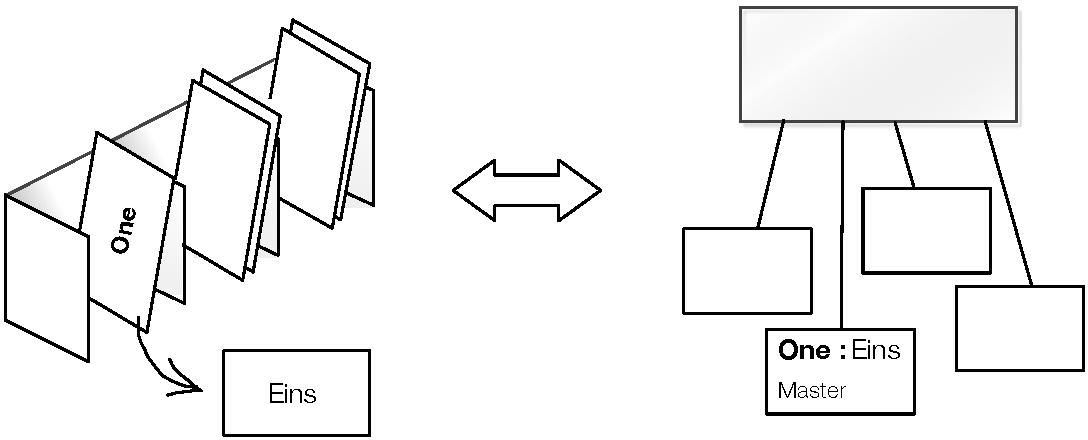
\includegraphics[width=\textwidth]{TGGTransformationExample.pdf}
  \caption{Transformation Goal}
  \label{fig:transformIdea}
\end{center}
\end{figure}

To briefly explain, each card in the box has a keyword on one side that a user can see, paired with a definition hidden on the opposite side. We could combine
each of these to create the keyword and content of a single dictionary entry, perhaps assigning a difficulty level based on its current position in the
box. The new entry can then be inserted anywhere. We also hope to be able to transform in the opposite direction, changing each
entry into a card by splitting up the contents, and inserting the new element into a specific partition in Box. After a short introduction to TGGs and setting
up your workspace correctly, we will then introduce and develop your first bidirectional transformation!

